\section{Data: from bytes on disk to a batch tensor}
\label{sec:data}

\subsection{Raw CIFAR-10 as torchvision hands it over}

\begin{repo}[\texttt{torchvision.datasets.CIFAR10(root="data", train=..., download=True)}]
The dataset object exposes two plain attributes, and the repo uses them directly. It never goes through torchvision's transforms or its \code{\_\_getitem\_\_}:
\begin{itemize}[nosep]
  \item \code{data.data}: a NumPy array of shape \shp{50000,32,32,3} for \code{train=True} or \shp{10000,32,32,3} for \code{train=False}, \code{dtype=uint8}, values $0..255$, channel order RGB, layout \emph{HWC}.
  \item \code{data.targets}: a Python \code{list} of 50{,}000 (or 10{,}000) integers in $0..9$.
\end{itemize}
Class indices: 0~airplane, 1~automobile, 2~bird, 3~cat, 4~deer, 5~dog, 6~frog, 7~horse, 8~ship, 9~truck. Training has 5{,}000 images per class and test has 1{,}000 per class.
\end{repo}

\begin{center}
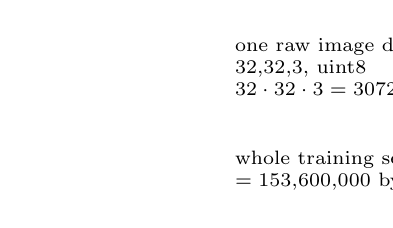
\begin{tikzpicture}
  \tensor{0}{0}{2.4}{2.4}{0.5}{cIn}{$W=32$ (axis 2)}{$H=32$ (axis 1)}{$3$ RGB (axis 3, \emph{last})}
  \node[font=\scriptsize,align=left,right] at (3.3,1.6) {one raw image \code{data.data[i]}\\ \shp{32,32,3}, \code{uint8}\\ $32\cdot32\cdot3 = 3072$ bytes};
  \node[font=\scriptsize,align=left,right] at (3.3,0.3) {whole training set: \shp{50000,32,32,3}\\ $=153{,}600{,}000$ bytes $\approx 146$\,MiB};
\end{tikzpicture}
\end{center}

\subsection{Train / validation split}

\begin{lstlisting}[firstnumber=5]
def split_indices(n,n_val,seed):
    g = torch.Generator()
    g.manual_seed(seed)
    result = torch.randperm(n=n,generator=g)
    validation_idx = result[:n_val]
    training_idx = result[n_val:]
    return training_idx,validation_idx
\end{lstlisting}

\begin{idea}
Draw one random permutation of $\{0,\dots,n-1\}$ and cut it: the first $n_\text{val}$ indices are validation and the rest are training. The two sets are disjoint and together cover everything. This is checked in \file{scripts/check\_split.py}: 45{,}000 + 5{,}000, zero overlap, same seed $\Rightarrow$ same split.
\end{idea}

\begin{repo}[two regimes]
\begin{itemize}[nosep]
  \item \textbf{Development} (default, used for all four ablation runs): \code{split\_indices(50000, 5000, 0)} gives 45{,}000 training and 5{,}000 validation indices, both \code{int64} tensors.
  \item \textbf{Final} (\code{--full}): \code{train\_idx = torch.arange(50000)}, with no validation set. The test set (10{,}000) is used only once, in \file{eval\_test.py}.
\end{itemize}
\end{repo}

\begin{warn}[the split seed is hard-coded]
\file{train\_resnet.py} calls \code{split\_indices(50000,5000,0)} with a literal \code{0}, not \code{args.seed}. Changing \code{--seed} changes the initialisation, the shuffling and the augmentation, but \emph{not} which 5{,}000 images are held out. This is deliberate: the 45k mean file \code{pixel\_mean\_45k\_seed0.npy} is only valid for that split.
\end{warn}

\subsection{Per-pixel mean}
\label{sec:mean}

\begin{lstlisting}[firstnumber=13]
def compute_pixel_mean(images,train_idx):
    training_images = images[train_idx.numpy()]
    floated_images = training_images.astype(np.float32)
    avg = floated_images.mean(axis=0)
    avg /= 255
    return avg
\end{lstlisting}

\begin{idea}[mean over images, not over pixels]
With $\mathcal T$ the set of training indices,
\[
  \mu[h,w,c] \;=\; \frac{1}{255\,|\mathcal T|}\sum_{i\in\mathcal T} x_i[h,w,c], \qquad \mu\in\R^{32\times32\times3}.
\]
This is a \emph{per-pixel, per-channel} mean: 3{,}072 separate numbers, an ``average image''. Contrast it with the more common \emph{per-channel} mean (3 numbers, the average over images \emph{and} positions). The paper says ``the per-pixel mean subtracted'', and that is what this repo implements.
\end{idea}

\begin{center}
\begin{tikzpicture}
  \foreach \k in {0,...,5} {\tensor{0.18*\k}{0.13*\k}{1.8}{1.8}{0.35}{cIn}{}{}{}}
  \node[font=\scriptsize] at (1.1,-0.35) {$|\mathcal T|$ images \shp{45000\text{ or }50000,32,32,3}};
  \draw[-{Stealth},thick] (3.2,1.2) -- (6.0,1.2) node[midway,above,font=\scriptsize]{\code{mean(axis=0)}} node[midway,below,font=\scriptsize]{$\div 255$};
  \tensor{6.6}{0.3}{1.8}{1.8}{0.35}{cK}{$32$}{$32$}{$3$}
  \node[font=\scriptsize,align=left,right] at (9.2,1.3) {$\mu$, \shp{32,32,3}, \code{float32}\\ values in $[0.392,\,0.550]$};
\end{tikzpicture}
\end{center}

\begin{repo}[the actual mean file \texttt{model/pixel\_mean\_50k.npy}]
Shape \shp{32,32,3}, \code{float32}, 12{,}416 bytes on disk (12{,}288 data + header). Averaged over positions, the three channels are $(0.4914,\;0.4822,\;0.4465)$, the familiar CIFAR-10 channel means. Individual entries range from $0.392$ to $0.550$; for example $\mu[0,0]=(0.513,0.534,0.520)$ at the top-left corner and $\mu[16,16]=(0.502,0.457,0.421)$ at the centre. The corner is greyer and the centre more reddish, which is where objects usually sit. Two files exist: \code{pixel\_mean\_45k\_seed0.npy} (development split) and \code{pixel\_mean\_50k.npy} (final model and service). The mean is always computed on the raw, \emph{un-augmented} training images.
\end{repo}

\begin{warn}[no division by a standard deviation]
\code{preprocess} subtracts the mean and does not divide by any standard deviation. The paper does not mention one either, and BN right after the stem rescales the activations anyway. Inputs therefore keep the raw $[0,1]$ spread, roughly $[-0.55,\,0.61]$ after centring.
\end{warn}

\subsection{Augmentation (training only)}
\label{sec:augment}

\begin{lstlisting}[firstnumber=20]
def augment(image,rng):
    padded_image = np.pad(image,pad_width=((4, 4), (4, 4), (0, 0)))
    top_offset = rng.integers(0,9)
    left_offset = rng.integers(0,9)
    cropped_image = padded_image[top_offset:top_offset+32, left_offset:left_offset+32, :]
    if rng.random() < 0.5 :
        cropped_image = np.ascontiguousarray(np.flip(cropped_image, axis=1))
    return cropped_image
\end{lstlisting}

\begin{center}
\begin{tikzpicture}[scale=0.11]
  % padded 40x40
  \fill[black!80] (0,0) rectangle (40,40);
  \fill[cIn] (4,4) rectangle (36,36);
  \draw (0,0) rectangle (40,40);
  \node[font=\tiny,white] at (20,2) {4 px zero (black) border};
  \node[font=\scriptsize] at (20,20) {original $32{\times}32$};
  \draw[warn,line width=1.2pt] (7,1) rectangle (39,33);
  \node[warn,font=\scriptsize,above] at (20,40) {crop window (orange): top $=7$, left $=7$};
  \node[below,font=\scriptsize] at (20,-1) {\shp{40,40,3} after \code{np.pad}};
  \draw[-{Stealth},thick] (46,17) -- (58,17) node[midway,above,font=\scriptsize]{slice};
  \fill[black!80] (60,1) rectangle (92,33);
  \fill[cIn] (60,4) rectangle (89,33);
  \draw (60,1) rectangle (92,33);
  \node[below,font=\scriptsize] at (76,0) {\shp{32,32,3} crop};
  \draw[-{Stealth},thick] (95,17) -- (107,17) node[midway,above,font=\scriptsize]{flip? $p{=}\frac12$};
  \fill[black!80] (110,1) rectangle (142,33);
  \fill[cIn] (113,4) rectangle (142,33);
  \draw (110,1) rectangle (142,33);
  \node[below,font=\scriptsize] at (126,0) {mirrored along width};
\end{tikzpicture}
\end{center}

\begin{idea}
Random translation by up to $\pm4$ pixels plus a random left--right mirror. The label stays the same, and the network sees a slightly different image every epoch. This is the standard ``pad 4, random crop 32, horizontal flip'' of the paper.
\end{idea}

\begin{repo}[exact behaviour]
\begin{itemize}[nosep]
  \item \code{np.pad} with no mode means constant \textbf{0}, applied to the \code{uint8} image, so the border is pure black \emph{before} normalisation.
  \item \code{rng.integers(0,9)} draws from $\{0,1,\dots,8\}$ (upper bound exclusive): 9 vertical $\times$ 9 horizontal offsets $=81$ crop positions, and offset 4 is the un-shifted image. With the flip, that gives up to $162$ distinct views of each image.
  \item \code{np.flip(axis=1)} reverses the \emph{width} axis of an HWC array, which is a horizontal mirror. \code{np.flip} returns a negative-stride view, so \code{np.ascontiguousarray} copies it into normal memory.
  \item Three random draws per image, in order: top offset, left offset, flip coin.
  \item \code{CIFARDataset} owns \emph{one} \code{np.random.default\_rng(seed)} created in \code{\_\_init\_\_}, used only when \code{train=True}. Its stream is consumed in the order the sampler requests images, so the whole augmentation sequence is reproducible given the seed.
\end{itemize}
\end{repo}

\begin{warn}[two subtle consequences]
\textbf{(1) Padding is not zero after preprocessing.} Pixels in the black border become $0/255-\mu[h,w,c]\approx(-0.49,-0.48,-0.45)$, not 0. The network sees ``black'', which is a legitimate image colour. It is \emph{not} the same as the zero padding inside the convolutions. Common pipelines that pad a PIL image before normalising behave the same way.

\textbf{(2) The RNG would be duplicated by worker processes.} With \code{DataLoader(num\_workers>0)}, each worker gets a copy of the same \code{rng} state, so different workers would produce identical augmentation sequences. The repo uses the default \code{num\_workers=0} (single process), so this does not happen. It is something to remember before ``speeding up'' the loader.
\end{warn}

\subsection{Preprocessing: the function shared by training and serving}
\label{sec:preprocess}

\begin{lstlisting}[firstnumber=29]
def preprocess(image,mean):
    image = image.astype(np.float32)
    image = image / 255
    image = image - mean
    tensored_image = torch.tensor(image)
    tensored_image = tensored_image.permute(2,0,1).contiguous()
    return tensored_image
\end{lstlisting}

\begin{center}
\begin{tikzpicture}
  \foreach \k/\xx/\lab/\top in {0/0/{\code{uint8}, $0..255$, HWC}/{raw},1/3.3/{\code{float32}, $0..255$}/{\code{astype}},2/6.6/{$[0,1]$}/{$\div 255$},3/9.9/{$\approx[-0.55,0.61]$}/{$-\,\mu$}} {
    \tensor{\xx}{0}{1.6}{1.6}{0.5}{cIn}{}{}{}
    \node[font=\scriptsize,below,align=center] at (\xx+0.8,-0.05) {\shp{32,32,3}\\\lab};
  }
  \foreach \xx/\op in {2.2/{\code{astype}},5.5/{$\div255$},8.8/{$-\,\mu$},12.1/{\code{permute}}}
    \draw[-{Stealth},thick] (\xx,0.8) -- (\xx+0.9,0.8) node[midway,above=3pt,font=\scriptsize,fill=white,inner sep=1pt]{\op};
  \tensor{13.5}{0}{1.6}{1.6}{0.5}{c16!40}{}{}{}
  \node[font=\scriptsize,below,align=center] at (14.3,-0.05) {\shp{3,32,32}\\CHW, for \code{Conv2d}};
\end{tikzpicture}
\end{center}

\begin{idea}[why the permute]
NumPy, PIL and torchvision store images channel-last (HWC). \code{nn.Conv2d} expects channel-first (CHW, and NCHW for a batch). \code{permute(2,0,1)} reorders the axes: new axis 0 = old axis 2 (channels), new 1 = old 0 (rows), new 2 = old 1 (columns). Mathematically, $X_\text{out}[c,h,w] = X_\text{in}[h,w,c]$. \code{permute} only changes strides, and \code{.contiguous()} materialises a copy laid out in the new order.
\end{idea}

\begin{repo}[broadcasting in $\text{image}-\mu$]
Both operands are \shp{32,32,3}, so the subtraction is element-wise with no broadcasting: each pixel subtracts \emph{its own} mean. Worked example from \file{samples/test0.png} (a cat): raw top-left pixel $(158,112,49)$, so $(0.6196,0.4392,0.1922)-(0.5126,0.5336,0.5198)=(0.1070,-0.0943,-0.3277)$, which is exactly \code{x[0,:,0,0]} in the model input. Over the whole image the values lie in $[-0.438,\,0.591]$ with mean $-0.048$.
\end{repo}

\subsection{Dataset and batching}

\begin{lstlisting}[firstnumber=37]
class CIFARDataset(torch.utils.data.Dataset):
    ...
    def __getitem__(self, i):
        idx = int(self.indices[i])
        image, label = self.images[idx], self.labels[idx]
        if self.train:
            image = augment(image=image,rng=self.rng)
        return preprocess(image, self.mean), label
\end{lstlisting}

\begin{idea}[indirection through \texttt{indices}]
The dataset never copies the images. It keeps the full array plus an index list, and position $i$ in the dataset maps to raw image \code{indices[i]}. The same object therefore serves the 45k split, the 5k split, the full 50k and the 10k test set.
\end{idea}

\begin{center}
\begin{tikzpicture}
  \foreach \k in {0,...,4} {\tensor{0.16*\k}{0.12*\k}{1.4}{1.4}{0.45}{c16!40}{}{}{}}
  \node[font=\scriptsize,align=center] at (1.0,-0.55) {128 samples, each\\ \shp{3,32,32} + an \code{int}};
  \draw[-{Stealth},thick] (2.9,1.1) -- (5.0,1.1) node[midway,above,font=\scriptsize]{default \code{collate}} node[midway,below,font=\scriptsize]{\code{torch.stack}};
  \tensor{5.4}{0.2}{1.4}{1.4}{2.2}{c16!40}{}{}{}
  \node[font=\scriptsize,align=center] at (6.7,-0.55) {batch axis 0 stacked\\ into the depth here};
  \node[font=\scriptsize,align=left,right] at (9.3,1.5) {$X$: \shp{128,3,32,32}, \code{float32}, 1.5\,MiB};
  \node[font=\scriptsize,align=left,right] at (9.3,0.7) {$y$: \shp{128}, \code{int64} (from Python \code{int}s)};
\end{tikzpicture}
\end{center}

\begin{repo}[loaders and the number of batches]
\begin{itemize}[nosep]
  \item Training: \code{DataLoader(batch\_size=128, shuffle=True, generator=g)} with \code{g} seeded by \code{--seed}. A new random order is drawn from \code{g} every epoch. \code{drop\_last} is \code{False}, so the remainder forms a short final batch.
  \item Validation and test: \code{shuffle=False}, \code{train=False}, so there is no augmentation.
\end{itemize}
\begin{center}
\begin{tabular}{@{}lrrrr@{}}
\toprule
set & images & full batches & last batch & batches per pass\\
\midrule
final training (50k) & 50{,}000 & 390 & 80 & \textbf{391}\\
development training (45k) & 45{,}000 & 351 & 72 & \textbf{352}\\
validation & 5{,}000 & 39 & 8 & 40\\
test & 10{,}000 & 78 & 16 & 79\\
\bottomrule
\end{tabular}
\end{center}
These numbers fix the epoch arithmetic of \cref{sec:schedule}: one epoch on 50k is 391 \emph{iterations}, and the schedule counts iterations, not epochs.
\end{repo}
